% Figure fragments; requires \usepackage{graphicx}.
% Paths below assume the main manuscript is compiled from the project root.
% Adapt paths when copying the two PDFs to a journal submission folder.
% The fragments have not been LaTeX-compiled in this environment.

\begin{figure}[tbp]
  \centering
  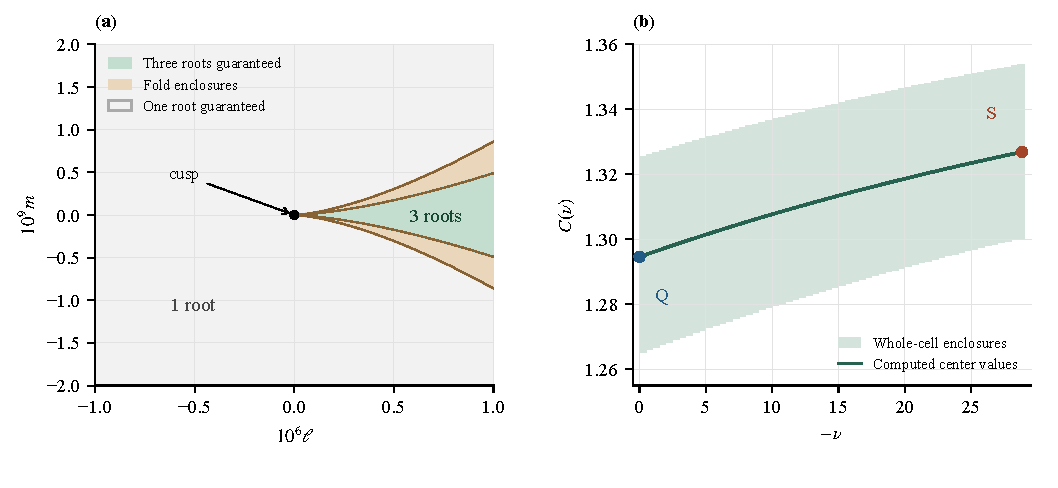
\includegraphics[width=\textwidth]{research/cusp_width/output/pdf/figure_1_cusp_geometry.pdf}
  \caption{Uniform local cusp geometry in exact-cusp-centered coordinates
  $s=t-t_*(\nu)$, $\ell=\lambda-\lambda_*(\nu)$ and
  $m=\mu-\mu_*(\nu)$, for $-29\leq\nu\leq0$.
  (a) Common root-count regions for $|s|\leq0.003$,
  $|\ell|\leq10^{-6}$ and $|m|\leq2\times10^{-9}$.
  The inner region has three simple real roots. The exterior has one,
  away from the discriminant; the cusp has one triple root.
  The intermediate bands enclose the folds, using
  $0.49\ell^{3/2}\leq|m_{\rm fold}|\leq0.86\ell^{3/2}$;
  within these bands the root count depends on the actual fold position.
  (b) The leading width coefficient
  $C(\nu)=-(8\sqrt{2}/3)D_3/D_4$ at the cusp.
  Shading gives enclosures over whole driver cells. The line connects
  computed center values and is a visual aid; the strict sign $C'(\nu)<0$
  is established by the separate interval proof. Points Q and S denote
  the exact quartic and sextic reference cusps, respectively.
  Figures are generated from the accompanying verification package.}
  \label{fig:r05-cusp-geometry}
\end{figure}

\begin{figure}[tbp]
  \centering
  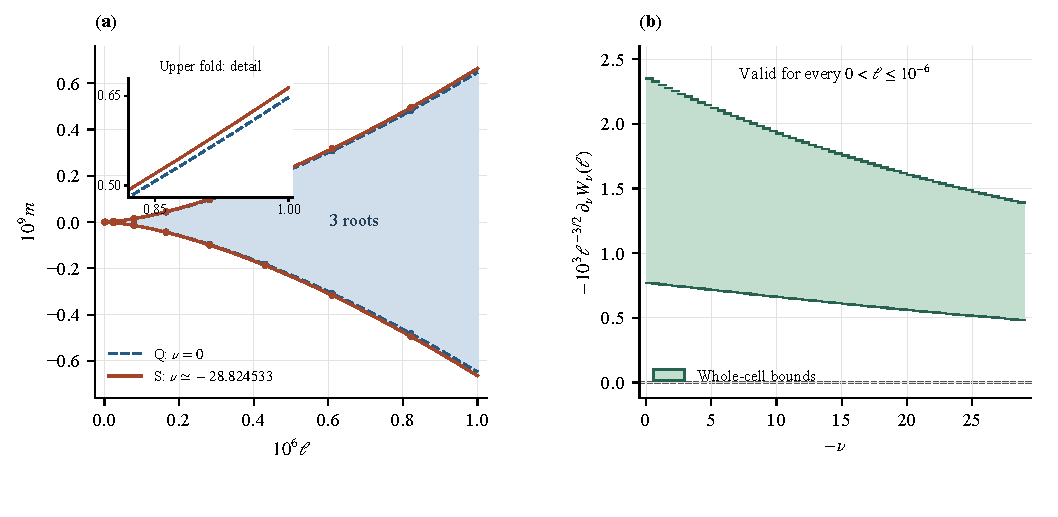
\includegraphics[width=\textwidth]{research/cusp_width/output/pdf/figure_2_finite_width.pdf}
  \caption{Finite fold motion and three-root width.
  (a) Fold sections at Q ($\nu=0$, dashed) and S
  ($\nu=\nu_S\simeq-28.82453269539050$, solid), each translated by its
  own exact cusp. Both sections use the same $\lambda,\mu$ control
  directions; the S section fixes $\nu$ and permits $\mu$ perturbations.
  The region between each pair of folds contains exactly three simple
  real roots in $|t-t_*(\nu)|\leq0.003$.
  Each pair is sampled at $\ell=10^{-6}(k/32)^2$, $k=1,\ldots,32$;
  all 128 fold points have validated root boxes, smaller than the plotted
  symbols. Selected symbols are displayed. Connecting lines and fills
  interpolate the samples for illustration. The inset magnifies the
  upper fold. At $\ell=10^{-6}$ the relative width increase from Q to S
  lies between $2.49463101\%$ and $2.49463103\%$.
  (b) Generating interval enclosures for
  $-10^3\ell^{-3/2}\partial_\nu W_\nu(\ell)$, valid for every
  $0<\ell\leq10^{-6}$ and every $\nu$ in each driver cell.
  These rectangles are uniform bounds, not samples of one graph.
  Their positive lower edges, together with the analytic transport
  identities, establish finite-width monotonicity. The proof separately
  establishes outward motion of both folds, hence strict nesting in
  the centered controls. An independent rational checker also verifies
  the positive sign and the conservative unscaled bounds
  $0.0003<-\ell^{-3/2}\partial_\nu W_\nu(\ell)<0.003$.}
  \label{fig:r05-finite-width}
\end{figure}
